\section{Objective and Methodology}
\label{sec:objective-methodology}

\subsection{Project Objective}
This project develops machine learning models to automatically classify internet images as advertisements or non-advertisements. This binary classification addresses the challenge of distinguishing advertising content from regular content, which is essential for:

\begin{itemize}
    \item \textbf{Content filtering}: Automatically detecting advertisement content
    \item \textbf{User experience}: Reducing intrusive advertising
    \item \textbf{Digital analysis}: Understanding advertisement patterns
    \item \textbf{Content moderation}: Supporting automated systems
\end{itemize}

With 1,559 features and class imbalance in our dataset, we aim to:
\begin{enumerate}
    \item Build models that handle high-dimensional data effectively
    \item Compare different machine learning approaches
    \item Identify key features for advertisement classification
    \item Provide practical implementation insights
\end{enumerate}

\subsection{Theoretical Foundation}
\subsubsection{Binary Classification Overview}
Our task is a \textbf{binary classification problem} where we predict one of two classes: advertisement (1) or non-advertisement (0). Given input features $\mathbf{x}$ (1,559 dimensions), we want to learn a function $f(\mathbf{x}) \rightarrow \{0,1\}$ that makes accurate predictions.

\textbf{Goal}: Minimize classification errors by learning patterns from training data.

\subsubsection{Evaluation Metrics}
We use multiple metrics to assess model performance, especially important for imbalanced datasets:

\textbf{Accuracy}: Overall correctness
\begin{equation}
Accuracy = \frac{\text{Correct Predictions}}{\text{Total Predictions}} = \frac{TP + TN}{TP + TN + FP + FN}
\end{equation}

\textbf{Precision}: How many predicted ads are actually ads
\begin{equation}
Precision = \frac{TP}{TP + FP}
\end{equation}

\textbf{Recall}: How many actual ads we correctly identified
\begin{equation}
Recall = \frac{TP}{TP + FN}
\end{equation}

\textbf{F1-Score}: Balance between Precision and Recall
\begin{equation}
F1 = 2 \cdot \frac{Precision \times Recall}{Precision + Recall}
\end{equation}

where TP=True Positives, TN=True Negatives, FP=False Positives, FN=False Negatives.

\subsubsection{Key Concepts}
\textbf{Bias-Variance Tradeoff}: Every model faces a balance between:
\begin{itemize}
    \item \textbf{Bias}: Error from oversimplifying (underfitting)
    \item \textbf{Variance}: Error from being too sensitive to training data (overfitting)
\end{itemize}

\textbf{Cross-Validation}: We split data into k parts, train on k-1 parts, test on 1 part, repeat k times. This gives reliable performance estimates and helps select best parameters.

\subsection{Machine Learning Methods}
We employ three different approaches, each representing distinct learning paradigms:

\subsubsection{k-Nearest Neighbors (k-NN)}
\textbf{Core Idea}: Classify new data points based on the majority class of their k closest neighbors.

\textbf{How it works}:
\begin{enumerate}
    \item Store all training data (\textbf{lazy learning})
    \item For a new point, find k nearest neighbors using distance
    \item Assign the most common class among these k neighbors
\end{enumerate}

\begin{figure}[h]
\centering
\vspace{0.3cm}
\includegraphics[width=0.5\textwidth]{graphics/knn_illustration.png}
\vspace{0.4cm}
\caption{k-NN Classification Example with k=3 Nearest Neighbors}
\vspace{1cm}
\end{figure}

\textbf{Key Distance Formulas}:
\begin{itemize}
    \item \textbf{Euclidean}: $d = \sqrt{\sum_{i=1}^{p} (x_i - y_i)^2}$ (straight-line distance)
    \item \textbf{Manhattan}: $d = \sum_{i=1}^{p} |x_i - y_i|$ (city-block distance)
\end{itemize}

\textbf{Advantages}:
\begin{itemize}
    \item Simple to understand and implement
    \item No assumptions about data distribution
    \item Works well with sufficient training data
\end{itemize}

\textbf{Challenges}:
\begin{itemize}
    \item Slow prediction (must check all training points)
    \item Sensitive to irrelevant features
    \item Struggles with high dimensions (curse of dimensionality)
\end{itemize}

\subsubsection{Decision Tree}
\textbf{Core Idea}: Create a tree of yes/no questions to classify data, like a flowchart.

\textbf{How it works}:
\begin{enumerate}
    \item Start with all training data at the root
    \item Find the best feature and threshold to split data
    \item Repeat for each branch until stopping criteria met
    \item Make predictions by following the path from root to leaf
\end{enumerate}

\begin{figure}[h]
\centering
\vspace{0.5cm}
\begin{tikzpicture}[
    scale=1.2,
    level 1/.style={sibling distance=4.5cm, level distance=3cm},
    level 2/.style={sibling distance=2.5cm, level distance=3cm},
    decision/.style={circle, draw=blue!60, thick, minimum size=1.8cm, 
                    text width=1.6cm, align=center, font=\small\bfseries,
                    fill=blue!20, 
                    drop shadow={opacity=0.3, shadow xshift=2pt, shadow yshift=-2pt}},
    leaf/.style={rectangle, draw=green!60, thick, minimum size=1.5cm, 
                text width=1.8cm, align=center, font=\small\bfseries,
                fill=green!20, rounded corners=8pt,
                drop shadow={opacity=0.3, shadow xshift=2pt, shadow yshift=-2pt}},
    edge from parent/.style={draw=gray!70, very thick, -stealth}
]
    \node[decision] {Feature A\\$> 0.5$?}
        child {
            node[decision] {Feature B\\$> 0.3$?}
            child {
                node[leaf] {\textbf{Non-Ad}\\(85\%)}
                edge from parent node[left, font=\footnotesize, text=red!70] {\textbf{No}}
            }
            child {
                node[leaf] {\textbf{Ad}\\(92\%)}
                edge from parent node[right, font=\footnotesize, text=green!70] {\textbf{Yes}}
            }
            edge from parent node[left, font=\footnotesize, text=red!70] {\textbf{No}}
        }
        child {
            node[leaf] {\textbf{Ad}\\(78\%)}
            edge from parent node[right, font=\footnotesize, text=green!70] {\textbf{Yes}}
        };
\end{tikzpicture}
\vspace{0.3cm}
\caption{Decision Tree Example for Ad Classification}
\vspace{1cm}
\end{figure}

\textbf{Key Concepts}:
\begin{itemize}
    \item \textbf{Gini Impurity}: Measures how "mixed" classes are in a node
    \begin{equation}
    Gini = 1 - \sum_{i=1}^{c} p_i^2
    \end{equation}
    \item \textbf{Information Gain}: How much a split reduces uncertainty
    \item \textbf{Pruning}: Removing branches to prevent overfitting
\end{itemize}

\textbf{Advantages}:
\begin{itemize}
    \item Easy to understand and interpret (white box)
    \item Handles both numerical and categorical features
    \item No need for feature scaling
    \item Automatically selects important features
\end{itemize}

\textbf{Challenges}:
\begin{itemize}
    \item Prone to overfitting (memorizing training data)
    \item Unstable (small data changes = different trees)
    \item Can create overly complex rules
\end{itemize}

\subsubsection{Random Forest}
\textbf{Core Idea}: Combine many decision trees to make better predictions (\textbf{ensemble method}).

\textbf{How it works}:
\begin{enumerate}
    \item Create many different training datasets using \textbf{bootstrap sampling} (random sampling with replacement)
    \item Train one decision tree on each dataset
    \item For each tree, use only a random subset of features at each split
    \item Combine all tree predictions by \textbf{majority voting}
\end{enumerate}

\begin{figure}[h]
\centering
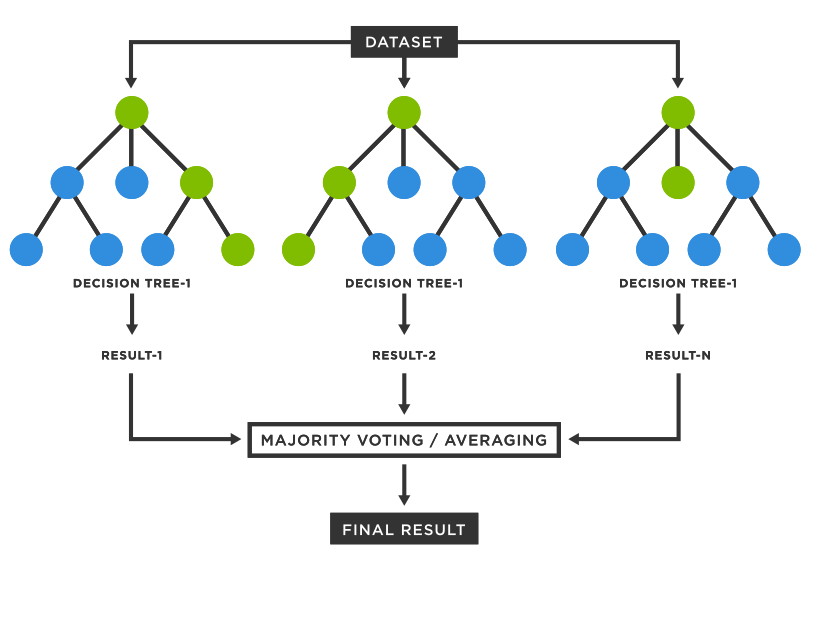
\includegraphics[width=0.8\textwidth]{graphics/random-forest-diagram.png}
\caption{Random Forest: Ensemble of Decision Trees for Ad Classification}
\vspace{1cm}
\end{figure}

\textbf{Key Features}:
\begin{itemize}
    \item \textbf{Bootstrap Sampling}: Each tree sees different data
    \item \textbf{Feature Randomness}: Each split uses random feature subset
    \item \textbf{Majority Voting}: Final prediction = most common prediction
    \item \textbf{Out-of-Bag Error}: Built-in validation using unused samples
\end{itemize}

\textbf{Why it works better}:
\begin{itemize}
    \item Individual trees may overfit, but averaging reduces this
    \item Different trees make different mistakes
    \item Combines strengths while canceling weaknesses
\end{itemize}

\textbf{Advantages}:
\begin{itemize}
    \item Excellent performance with high-dimensional data
    \item Provides feature importance automatically
    \item Robust to overfitting
    \item Handles missing data well
    \item Less parameter tuning needed
\end{itemize}

\textbf{Challenges}:
\begin{itemize}
    \item Less interpretable than single trees (black box)
    \item Computationally expensive with many trees
    \item Memory intensive for large datasets
\end{itemize}

\subsection{Our Approach}
We follow a systematic process:

\begin{enumerate}
    \item \textbf{Data Preparation}: 
    \begin{itemize}
        \item Normalize features (important for k-NN)
        \item Split data: 70\% training, 30\% testing
        \item Handle class imbalance
    \end{itemize}
    
    \item \textbf{Model Training}:
    \begin{itemize}
        \item k-NN: Find best k value using cross-validation
        \item Decision Tree: Use pruning to prevent overfitting
        \item Random Forest: Tune number of trees and features per split
    \end{itemize}
    
    \item \textbf{Evaluation}:
    \begin{itemize}
        \item Compare using Accuracy, Precision, Recall, F1-score
        \item Analyze confusion matrices
        \item Examine feature importance (from Random Forest)
    \end{itemize}
\end{enumerate}

\subsection{Expected Results}
This study will:
\begin{itemize}
    \item Identify the best method for ad classification
    \item Discover which features are most important for detecting ads
    \item Provide practical recommendations for real-world systems
    \item Show how ensemble methods handle high-dimensional data
\end{itemize}

By comparing three different approaches, we ensure robust conclusions about the most effective techniques for internet advertisement classification.